\documentclass[a4paper, 11pt]{article}
\usepackage{amsmath}
\usepackage{graphicx}
\usepackage{geometry}
\usepackage{listings}
\usepackage{xcolor}
\usepackage{float}
\usepackage[colorlinks,linkcolor=red]{hyperref}
\geometry{scale=0.8}
\usepackage[UTF8]{ctex}


\title{	
\normalfont \normalsize
\textsc{School of Data and Computer Science, Sun Yat-sen University} \\ [25pt] %textsc small capital letters
\rule{\textwidth}{0.5pt} \\[0.4cm] % Thin top horizontal rule
\huge  E14 BP Algorithm (C++/Python)\\ % The assignment title
\rule{\textwidth}{2pt} \\[0.5cm] % Thick bottom horizontal rule
\author{18340052  何泽}
\date{\normalsize\today}
}

\begin{document}
\maketitle
\tableofcontents
\newpage
\section{Horse Colic Data Set}
The description of the horse colic data set (\url{http://archive.ics.uci.edu/ml/datasets/Horse+Colic}) is as follows:
\begin{figure}[ht]
\centering
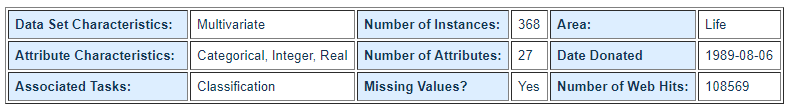
\includegraphics[width=15cm]{horse}
\end{figure}

We aim at trying to predict if a horse with colic will live or die.

Note that we should deal with missing values in the data! Here are some options:
\begin{itemize}
	\item Use the feature’s mean value from all the available data.
	\item Fill in the unknown with a special value like -1.
	\item Ignore the instance.
	\item Use a mean value from similar items.
	\item Use another machine learning algorithm to predict the value.
\end{itemize}

\section{Reference Materials}
\begin{enumerate}
	\item Stanford: \textbf{CS231n: Convolutional Neural Networks for Visual Recognition} by Fei-Fei Li,etc.
	\begin{itemize}
		\item Course website: \url{http://cs231n.stanford.edu/2017/syllabus.html}
		\item Video website: \url{https://www.bilibili.com/video/av17204303/?p=9&tdsourcetag=s_pctim_aiomsg}
	\end{itemize}
	
	\item \textbf{Machine Learning} by Hung-yi Lee
	\begin{itemize}
		\item Course website: \url{http://speech.ee.ntu.edu.tw/~tlkagk/index.html}
		\item Video website: \url{https://www.bilibili.com/video/av9770302/from=search}
	\end{itemize}
	\item A Simple neural network code template
\lstset{
	columns=fixed,       
	numbers=left,                                        % 在左侧显示行号
	frame=shadowbox,                                          % 不显示背景边框
	backgroundcolor=\color[RGB]{245,245,244},            % 设定背景颜色
	keywordstyle=\color[RGB]{0,92,230},                 % 设定关键字颜色
	numberstyle=\footnotesize\color{darkgray},           % 设定行号格式
	commentstyle=\it\color[RGB]{0,96,96},                % 设置代码注释的格式
	stringstyle=\rmfamily\slshape\color[RGB]{230,92,0},   % 设置字符串格式
	showstringspaces=false,                              % 不显示字符串中的空格
	breaklines,
	language=Python,      
}
	\begin{lstlisting}
# -*- coding: utf-8 -*
import random
import math

# Shorthand:
# "pd_" as a variable prefix means "partial derivative"
# "d_" as a variable prefix means "derivative"
# "_wrt_" is shorthand for "with respect to"
# "w_ho" and "w_ih" are the index of weights from hidden to output layer neurons and input to hidden layer neurons respectively

class NeuralNetwork:
    LEARNING_RATE = 0.5
    def __init__(self, num_inputs, num_hidden, num_outputs, hidden_layer_weights = None, hidden_layer_bias = None, output_layer_weights = None, output_layer_bias = None):
    #Your Code Here

    def init_weights_from_inputs_to_hidden_layer_neurons(self, hidden_layer_weights):
    #Your Code Here

    def init_weights_from_hidden_layer_neurons_to_output_layer_neurons(self, output_layer_weights):    
    #Your Code Here

    def inspect(self):
        print('------')
        print('* Inputs: {}'.format(self.num_inputs))
        print('------')
        print('Hidden Layer')
        self.hidden_layer.inspect()
        print('------')
        print('* Output Layer')
        self.output_layer.inspect()
        print('------')

    def feed_forward(self, inputs):
        #Your Code Here

    # Uses online learning, ie updating the weights after each training case
    def train(self, training_inputs, training_outputs):
        self.feed_forward(training_inputs)

        # 1. Output neuron deltas        
        #Your Code Here
        # ∂E/∂zⱼ       

        # 2. Hidden neuron deltas        
        # We need to calculate the derivative of the error with respect to the output of each hidden layer neuron
        # dE/dyⱼ = Σ ∂E/∂zⱼ * ∂z/∂yⱼ = Σ ∂E/∂zⱼ * wᵢⱼ
        # ∂E/∂zⱼ = dE/dyⱼ * ∂zⱼ/∂
        #Your Code Here

        # 3. Update output neuron weights
        # ∂Eⱼ/∂wᵢⱼ = ∂E/∂zⱼ * ∂zⱼ/∂wᵢⱼ             
        # Δw = α * ∂Eⱼ/∂wᵢ
        #Your Code Here        

        # 4. Update hidden neuron weights
        # ∂Eⱼ/∂wᵢ = ∂E/∂zⱼ * ∂zⱼ/∂wᵢ    
        # Δw = α * ∂Eⱼ/∂wᵢ
        #Your Code Here
                
    def calculate_total_error(self, training_sets):
        #Your Code Here
        return total_error

class NeuronLayer:
    def __init__(self, num_neurons, bias):

        # Every neuron in a layer shares the same bias
        self.bias = bias if bias else random.random()

        self.neurons = []
        for i in range(num_neurons):
            self.neurons.append(Neuron(self.bias))

    def inspect(self):
        print('Neurons:', len(self.neurons))
        for n in range(len(self.neurons)):
            print(' Neuron', n)
            for w in range(len(self.neurons[n].weights)):
                print('  Weight:', self.neurons[n].weights[w])
            print('  Bias:', self.bias)

    def feed_forward(self, inputs):
        outputs = []
        for neuron in self.neurons:
            outputs.append(neuron.calculate_output(inputs))
        return outputs

    def get_outputs(self):
        outputs = []
        for neuron in self.neurons:
            outputs.append(neuron.output)
        return outputs

class Neuron:
    def __init__(self, bias):
        self.bias = bias
        self.weights = []

    def calculate_output(self, inputs):
    #Your Code Here

    def calculate_total_net_input(self):
    #Your Code Here

    # Apply the logistic function to squash the output of the neuron
    # The result is sometimes referred to as 'net' [2] or 'net' [1]
    def squash(self, total_net_input):
    #Your Code Here

    # Determine how much the neuron's total input has to change to move closer to the expected output
    #
    # Now that we have the partial derivative of the error with respect to the output (∂E/∂yⱼ) and
    # the derivative of the output with respect to the total net input (dyⱼ/dzⱼ) we can calculate
    # the partial derivative of the error with respect to the total net input.
    # This value is also known as the delta (δ) [1]
    # δ = ∂E/∂zⱼ = ∂E/∂yⱼ * dyⱼ/dzⱼ
    #
    def calculate_pd_error_wrt_total_net_input(self, target_output):
    #Your Code Here

    # The error for each neuron is calculated by the Mean Square Error method:
    def calculate_error(self, target_output):
    #Your Code Here

    # The partial derivate of the error with respect to actual output then is calculated by:
    # = 2 * 0.5 * (target output - actual output) ^ (2 - 1) * -1
    # = -(target output - actual output)
    #
    # The Wikipedia article on backpropagation [1] simplifies to the following, but most other learning material does not [2]
    # = actual output - target output
    #
    # Alternative, you can use (target - output), but then need to add it during backpropagation [3]
    #
    # Note that the actual output of the output neuron is often written as yⱼ and target output as tⱼ so:
    # = ∂E/∂yⱼ = -(tⱼ - yⱼ)
    def calculate_pd_error_wrt_output(self, target_output):
    #Your Code Here

    # The total net input into the neuron is squashed using logistic function to calculate the neuron's output:
    # yⱼ = φ = 1 / (1 + e^(-zⱼ))
    # Note that where ⱼ represents the output of the neurons in whatever layer we're looking at and ᵢ represents the layer below it
    #
    # The derivative (not partial derivative since there is only one variable) of the output then is:
    # dyⱼ/dzⱼ = yⱼ * (1 - yⱼ)
    def calculate_pd_total_net_input_wrt_input(self):
    #Your Code Here

    # The total net input is the weighted sum of all the inputs to the neuron and their respective weights:
    # = zⱼ = netⱼ = x₁w₁ + x₂w₂ ...
    #
    # The partial derivative of the total net input with respective to a given weight (with everything else held constant) then is:
    # = ∂zⱼ/∂wᵢ = some constant + 1 * xᵢw₁^(1-0) + some constant ... = xᵢ
    def calculate_pd_total_net_input_wrt_weight(self, index):
    #Your Code Here

# An example:

nn = NeuralNetwork(2, 2, 2, hidden_layer_weights=[0.15, 0.2, 0.25, 0.3], hidden_layer_bias=0.35, output_layer_weights=[0.4, 0.45, 0.5, 0.55], output_layer_bias=0.6)
for i in range(10000):
    nn.train([0.05, 0.1], [0.01, 0.99])
    print(i, round(nn.calculate_total_error([[[0.05, 0.1], [0.01, 0.99]]]), 9))


	\end{lstlisting}

\end{enumerate}
\section{Tasks}
\begin{itemize}
	\item Given the training set \texttt{horse-colic.data} and the testing set \texttt{horse-colic.test}, implement the BP algorithm and establish a neural network to predict if horses with colic will live or die. In addition, you should calculate the accuracy rate.
	\item Please submit a file named \texttt{E14\_YourNumber.pdf} and send it to \texttt{ai\_2020@foxmail.com}
	\item Draw the training loss and accuracy curves
	\item (optional) You can try different structure of neural network and compare their accuracy and the time they cost.
\end{itemize}
\section{Codes and Results}
\begin{enumerate}
	\item Result:

	\begin{figure}[H]
	  \centering
	  
\includegraphics[width=0.95\linewidth]{2.png}
	  \qquad
	\end{figure}
	\begin{figure}[H]
	  \centering
	  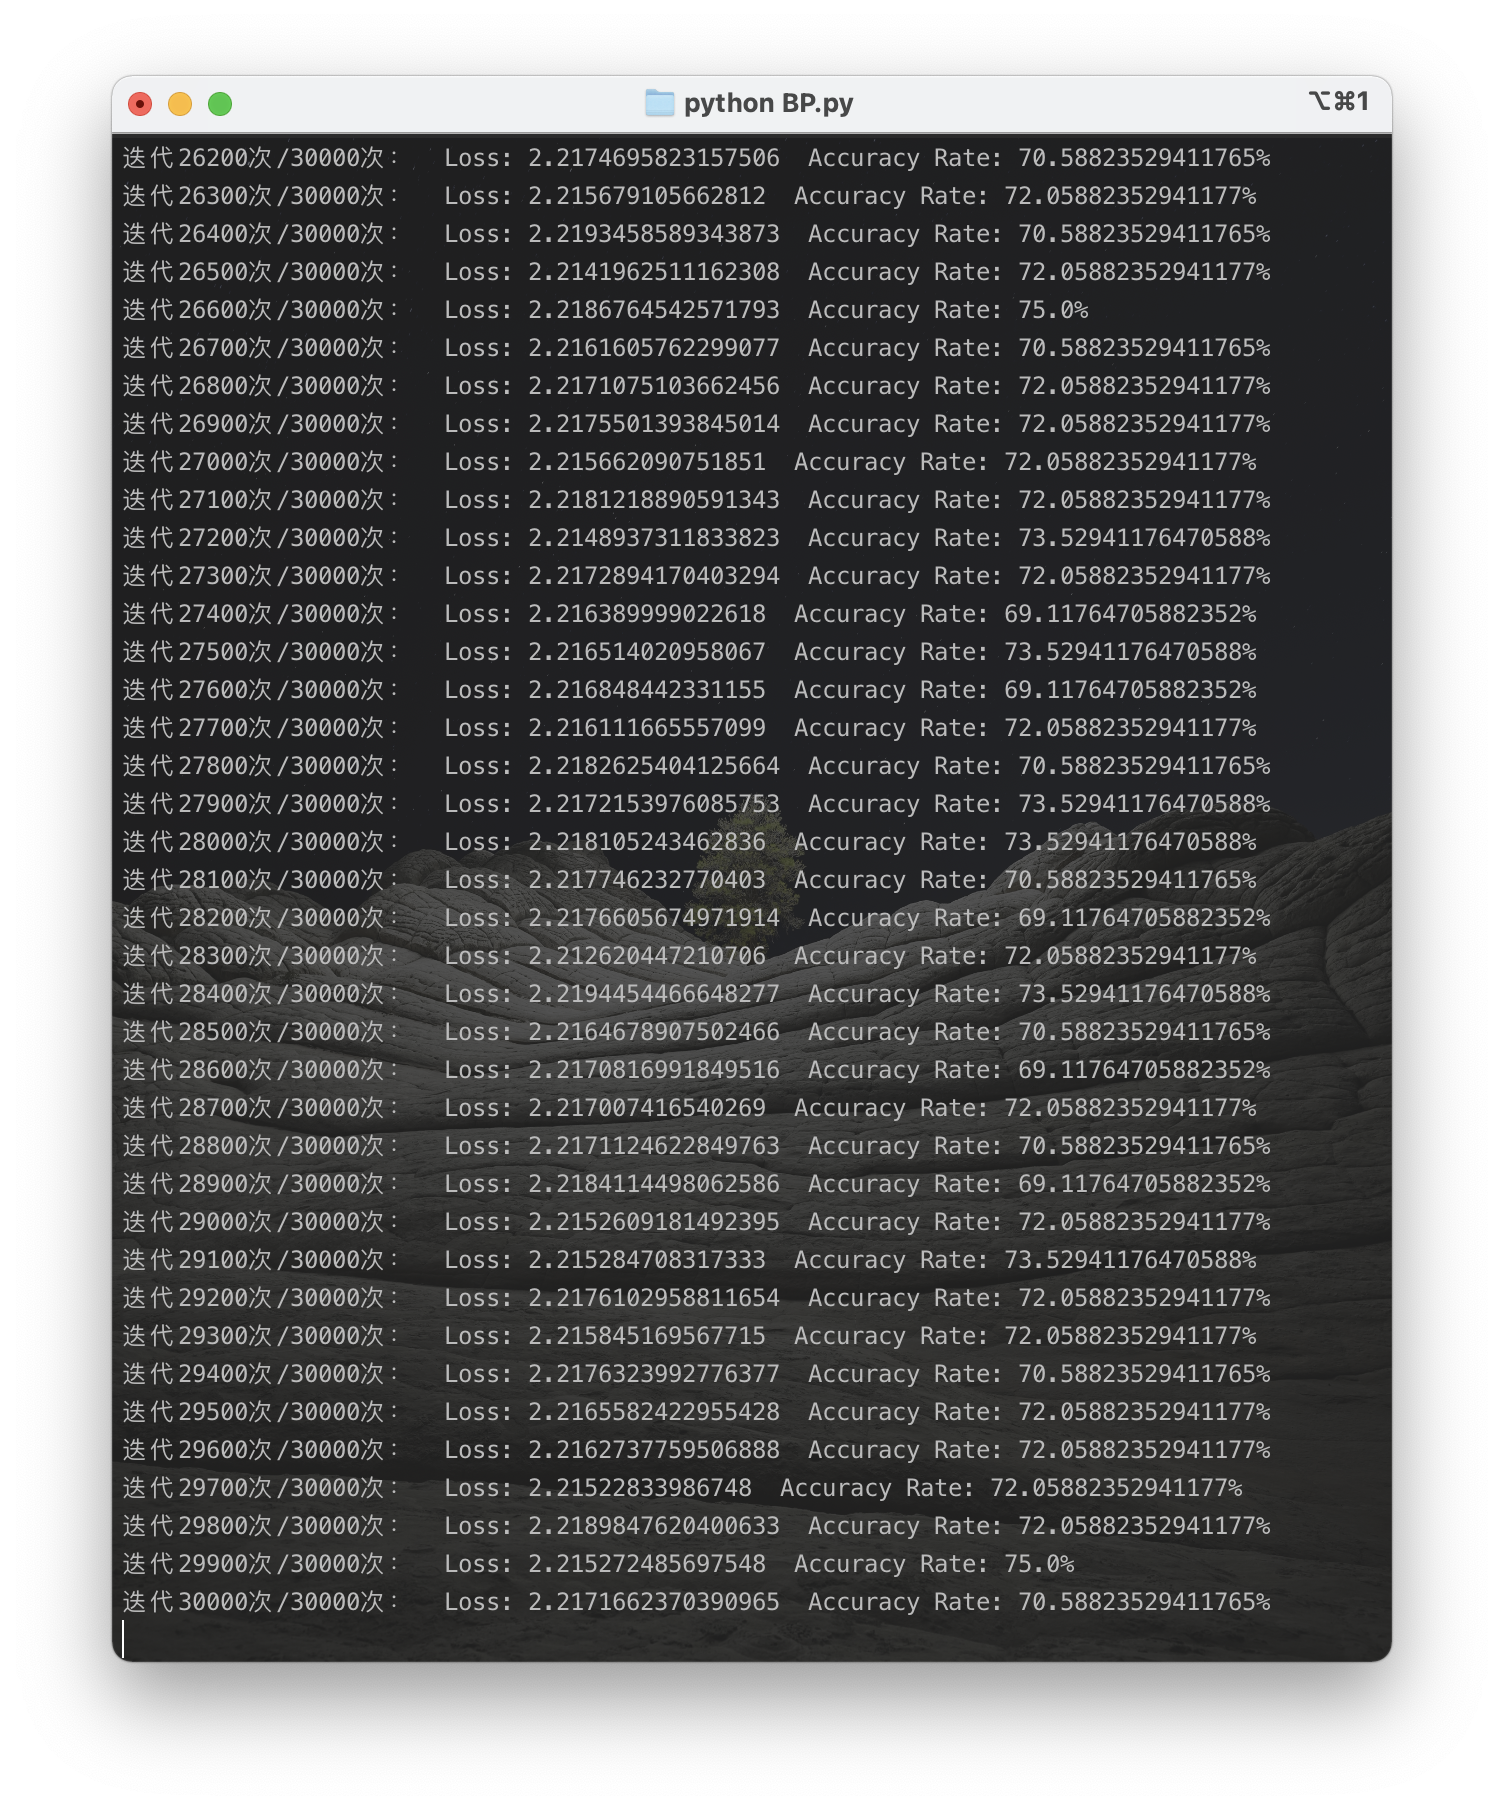
\includegraphics[width=0.9\linewidth]{1.png}
	  \qquad
	 \end{figure}
	\item Code:

\lstset{
	columns=fixed,       
	numbers=left,                                        % 在左侧显示行号
	frame=shadowbox,                                          % 不显示背景边框
	backgroundcolor=\color[RGB]{245,245,244},            % 设定背景颜色
	keywordstyle=\color[RGB]{0,92,230},                 % 设定关键字颜色
	numberstyle=\footnotesize\color{darkgray},           % 设定行号格式
	commentstyle=\it\color[RGB]{0,96,96},                % 设置代码注释的格式
	stringstyle=\rmfamily\slshape\color[RGB]{230,92,0},   % 设置字符串格式
	showstringspaces=false,                              % 不显示字符串中的空格
	breaklines,
	language=Python,      
}
\begin{lstlisting}
import pandas as pd
import numpy as np
import matplotlib.pyplot as plt

class NeuralNetwork(object):
    def __init__(self,in_features,hidden_features,out_features,learning_rate=0.1):
        self.fc1 = FullyConnectedLayer(in_features,hidden_features,True)
        self.fc2 = FullyConnectedLayer(hidden_features,out_features,True)
        self.learning_rate = learning_rate
        self.memory = {}
        self.train_flag = True

    def train(self):
        self.train_flag = True
        
    def eval(self):
        self.train_flag = False
        
    def relu(self,x):
        return np.maximum(0,x)

    def d_relu(self,x):
        x[x <= 0] = 0
        x[x > 0] = 1
        return x

    def sigmoid(self,x):
        return 1 / (1 + np.exp(-x))

    def d_sigmoid(self,x):
        return self.sigmoid(x) * (1 - self.sigmoid(x))

    def tanh(self,x):
        return np.tanh(x)

    def d_tanh(self,x):
        return 1 - np.tanh(x) ** 2

    def MSE(self,y_hat,y):
        return np.linalg.norm(y_hat - y)

    def cross_entropy(self,y_hat,y):
        return y * np.log(y_hat) + (1 - y) * np.log(1 - y_hat)

    def forward(self,x):
        if self.train_flag:
            self.memory["a0"] = np.copy(x)
            x = self.fc1(x)
            self.memory["z1"] = np.copy(x)
            x = self.sigmoid(x)
            self.memory["a1"] = np.copy(x)
            x = self.fc2(x)
            self.memory["z2"] = np.copy(x)
            x = self.sigmoid(x)
        else:
            x = self.fc1(x)
            x = self.sigmoid(x)
            x = self.fc2(x)
            x = self.sigmoid(x)
        return x

    def backward(self,y_hat,y,lamb=0):
        batch_size = y.shape[0]
        delta = [0] * 3
        delta[2] = (y_hat - y) * self.d_sigmoid(self.memory["z2"])
        delta[1] = np.dot(delta[2],self.fc2.weight) * self.d_sigmoid(self.memory["z1"]) 
        nabla_W = [0] * 2
        nabla_W[1] = np.einsum("ij,ik->ijk",delta[2],self.memory["a1"])
        nabla_W[0] = np.einsum("ij,ik->ijk",delta[1],self.memory["a0"])
        nabla_b = [0] * 2
        nabla_b[1] = delta[2]
        nabla_b[0] = delta[1]
        nabla_W[1] = nabla_W[1].mean(axis=0)
        nabla_W[0] = nabla_W[0].mean(axis=0)
        nabla_b[1] = nabla_b[1].mean(axis=0)
        nabla_b[0] = nabla_b[0].mean(axis=0)
        self.fc2.weight -= self.learning_rate * (nabla_W[1] + lamb * self.fc2.weight / batch_size)
        self.fc1.weight -= self.learning_rate * (nabla_W[0] + lamb * self.fc1.weight / batch_size)
        self.fc2.bias -= self.learning_rate * nabla_b[1]
        self.fc1.bias -= self.learning_rate * nabla_b[0]

class FullyConnectedLayer(object):
    def __init__(self, in_features, out_features, bias=True):
        self.in_features = in_features
        self.out_features = out_features
        self.weight = np.random.normal(0,np.sqrt(2/in_features),(out_features,in_features))
        if bias:
            self.bias = np.random.rand(out_features)
        else:
            self.bias = None
            
    def forward(self, inputs):
        if type(self.bias) != type(None):
            return np.dot(inputs, self.weight.T) + self.bias
        else:
            return np.dot(inputs, self.weight.T)
        
    def __call__(self,x):
        return self.forward(x)

def preprocessing(data):
    drop_attr = ["type of lesion 2", "type of lesion 3","Hospital Number","nasogastric reflux PH","abdomcentesis total protein"]
    attributes = []
    for a in data.columns.values:
        in_flag = attr_dict.get(a,None)
        if in_flag == None:
            attributes.append(a)
        elif in_flag == 0 and a not in drop_attr:
            attributes.append(a)
        else:
            pass
    df = data[attributes]
    return df

def fill_data(data):
    for a in data.columns.values:
        if a in ["type of lesion 1", "Hospital Number"]:
            continue
        if data[a].dtype != np.int64:
            have_data = data[data[a] != "?"][a]
            if attr_dict[a]:
                data.loc[data[a] == "?",a] = have_data.value_counts().idxmax() 
                if a != "outcome" and attr_dict[a] != 2:
                    data[a] = pd.Categorical(data[a])
                    dummies = pd.get_dummies(data[a],prefix="{}_category".format(a))
                    data = pd.concat([data,dummies],axis=1)
            else:
                data.loc[data[a] == "?",a] = np.mean(have_data.astype(np.float))
        elif attr_dict[a] == 1:
            data[a] = pd.Categorical(data[a])
            dummies = pd.get_dummies(data[a],prefix="{}_category".format(a))
            data = pd.concat([data,dummies],axis=1)
    return data.astype(np.float)

def get_batches(data,label,batch_size=1):
    num_batches = len(data) // batch_size
    for i in range(0,num_batches,batch_size):
        yield data[i:i+batch_size].to_numpy(), np.array(label[i:i+batch_size])

def test(net,test_X,test_y,flag=True,print_flag=False):
    cnt = 0
    for j, x in test_X.iterrows():
        net.eval()
        Y_hat = net.forward(x.to_numpy().reshape(1,-1))
        predicted = np.argmax(Y_hat) + 1
        y = test_y[j]
        if print_flag:
            print(Y_hat,predicted,y)
        if flag:
            if predicted == y:
                cnt += 1
        else:
            if [1 if t + 1 == predicted else 0 for t in range(3)] == y:
                cnt += 1
    return (cnt / len(test_X))

def train(net,max_iter=1000):
    loss_history, accuracy_history = [], []
    losses = []
    for i in range(max_iter):
        net.train()
        batches = get_batches(train_data,train_label,16)
        for x, y in batches:
            Y_hat = net.forward(x)
            loss = net.MSE(Y_hat, y)
            losses.append(loss)
            net.backward(Y_hat,y,0.1)
        if (i+1) % 100 == 0:
            avg_loss = np.array(losses).mean()
            loss_history.append(avg_loss)
            losses = []
            acc = test(net,test_data,test_label)
            accuracy_history.append(acc)
            print("迭代{}次/{}次:  Loss: {}  Accuracy Rate: {}%".format(i+1,max_iter,avg_loss,acc*100))
    return loss_history, accuracy_history


attr_dict = {"surgery": 1,
 "Age": 2,
 "Hospital Number": 1,
 "rectal temperature": 0,
 "pulse": 0,
 "respiratory rate": 0,
 "temperature of extremities": 2,
 "peripheral pulse": 2,
 "mucous membranes": 1,
 "capillary refill time": 2,
 "pain": 1,
 "peristalsis": 2,
 "abdominal distension": 1,
 "nasogastric tube": 1,
 "nasogastric reflux": 2,
 "nasogastric reflux PH": 0,
 "rectal examination": 2,
 "abdomen": 1,
 "packed cell volume": 0,
 "total protein": 0,
 "abdominocentesis appearance": 1,
 "abdomcentesis total protein": 0,
 "outcome": 1,
 "surgical lesion": 1,
 "type of lesion 1": 1,
 "type of lesion 2": 1,
 "type of lesion 3": 1,
 "cp_data": 1}

train_data = pd.read_csv("horse-colic.data",names=attr_dict.keys(),index_col=False,delim_whitespace=True)
test_data = pd.read_csv("horse-colic.test",names=attr_dict.keys(),index_col=False,delim_whitespace=True)
data = pd.concat([train_data,test_data],axis=0)
data = fill_data(data)
label = data["outcome"].astype(np.float)
train_label, test_label = label[:len(train_data)], label[len(train_data):]
train_label = [[1,0,0] if label == 1 else ([0,1,0] if label == 2 else [0,0,1]) for label in train_label]
data = preprocessing(data)
train_data, test_data = data[:len(train_data)], data[len(train_data):]

net = NeuralNetwork(len(train_data.columns.values),5,3,0.1)
loss_history, accuracy_history = train(net,30000)
fig = plt.figure()
ax = fig.add_subplot(111)
lns1 = ax.plot(loss_history,"-c",label="Loss")
ax2 = ax.twinx()
lns2 = ax2.plot(accuracy_history,"-b",label="Accuracy Rate")
lns = lns1 + lns2
labs = [l.get_label() for l in lns]
ax.legend(lns,labs,loc=0)
ax.set_xlabel("Iteration (x100)")
ax.set_ylabel("Loss")
ax2.set_ylabel("Accuracy Rate")
ax2.set_ylim(0,1)
plt.show()
\end{lstlisting}

\end{enumerate}

%\clearpage
%\bibliography{E:/Papers/LiuLab}
%\bibliographystyle{apalike}
\end{document} 
%%% Local Variables:
%%% mode: latex
%%% TeX-master: t
%%% End:
